% https://github.com/paraslonic/bacgenome_assembly <- may be add description of this

\section{Алгоритмизация подхода выявления оперонов, наличие которых ассоциировано с определенным признаком. } \label{chaptOperons}

\subsection{Проблема поиска генетических ассоциаций для субпопуляций бактерий}
Предположим, что у нас есть некоторый признак, по которому мы можем разбить набор геномов на группы, и наша задача - установить, какие гены значимо чаще (либо реже) встречаются в одной из групп. Распространенным подходом в подобном случае является оценка значимости по каждому отдельному гену. После проведения этих тестов необходимо применить поправку на множественное сравнение, так как иначе следует ожидать множество ложно положительных результатов. В случае, если работа ведется на данных о полной последовательности генома, имеется большое количество анализируемых генов (порядка $10^3 - 10^4$), а размеры групп, как правило, незначительны (порядка $10^1 - 10^2$), что приводит к тому, что после поправки на множественное сравнение, ни один из анализируемых генов не проходит даже низкие пороги на значимость. В качестве одного из способов преодоления описанной выше проблемы мы предложили использовать информацию об организации генов в опероны для поиска значимых ассоциаций \cite{rakitina2017genome}. Рассматривая оперон как структурную единицу, мы значительно сокращаем количество анализируемых признаков, так, что оно становится сравнимым с размерами групп.

\subsection{Алгоритм поиска генетических ассоциаций}
Первым шагом выполняется оценка значимости в точном тесте Фишера по каждому гену независимо. Затем ищутся опероны, в которых количество генов с заданным уровнем значимости выше, чем ожидается при случайном распределении генов по оперонам. Для оценки количества, ожидаемого при случайном распределении, применяется метод случайных перестановок либо оценка, основанная на распределении Пуассона. В первом случае, перестановки производятся в таблице соответствий генов и оперонов и подсчитывается максимальная доля значимых генов в оперонах данной длины. Во втором случае, на основе наблюдаемого количества генов с уровнем значимости превышающим пороговый, раcсчитывается их средняя плотность на единицу длины и затем для каждого оперона оценивается вероятность наблюдать данное либо большее количество подобных генов в соответствие с распределением Пуассона. И в первом, и во втором случае, финальным шагом является проведение поправки на множественное сравнение, но уже не для генов, а для оперонов, количество которых, как правило, значительно ниже общего количества генов.

Алгоритм первого подхода можно записать следующим образом:\\
Пусть $I$ - набор оперонов, определенный на референсном геноме $R$.
\begin{enumerate} 
  \item Определить группы ортологии $O$.
  \item Для каждой группы ортологии $o \in O $ имеющей хоть один ген, представленный в $R$, посчитать $P\textsubscript{o} = $p-value в точном тесте Фишера.
  \item Для каждого оперона $i \in I$ посчитать $Fobs\textsubscript{i} = $доля входящих в него генов, для которых $P\textsubscript{o} < 0.05$.
  \item Для каждого $j \in [1..10000]$
  	\begin{enumerate} 
        \item Провести случайную пермутацию значений $P$ .
        \item Для каждого оперона $i \in I$ посчитать $Frnd\textsubscript{i, j} = $доля генов, для которых $P\textsubscript{o} < 0.05$.
  	\end{enumerate} 
  \item Для каждого оперона $i \in I$ найти $Fmaxrnd\textsubscript{i}=max\textsubscript{j}(Frnd\textsubscript{i, j})$ - максимальную долю генов в опероне при случайных перестановках значений значимостей для генов.
  \item Для каждого оперона $i \in I$, если $Fobs\textsubscript{i}>Fmaxrnd\textsubscript{i}$, считать его значимым с уровнем значимости $p{}$.
\end{enumerate}

Перейдем к описанию результатов применения данного подхода.

\subsubsection{Поиск оперонов, значимо чаще встречающихся у изолятов бактерий \textit{E. coli}, изолированных от людей с болезнью Крона.}
В анализе был использован 51 геном \textit{E. coli}, из которых 27 были геномы бактерий, изолированных от больных с болезнью Крона, а 24 генома принадлежали изолятам, полученным от здоровых людей. При помощи программы OrthoFinder \cite{emms2015orthofinder} мы получили 11885 ортогрупп. Далее, при помощи точного теста Фишера, для каждой ортогруппы мы оценили статистическую значимость ее неравномерной представленности в группах. Минимальное значение p-value, при этом, было меньше, чем 0.00037, а медианное - 0.78. После поправки на множественные сравнения (метод Бенджамини-Хохберга \cite{benjamini1995controlling}) минимальное значение p\-value составляет 1 (такой же результат дают методы Бенджамини-Йекутили \cite{benjamini2001control} и Холма \cite{holm1979simple})). Код для проведения данного анализа доступен в репозитории \url{https://github.com/paraslonic/Rakitina_etal_Crohn_paper/blob/master/ogEnrichment/calcFDR.r}. 

Следующим шагом мы осуществили описанный выше тип анализа, для поиска значимо дифференциально представленных оперонов. Информация об оперонах была взята из базы данных DOORS \cite{mao2014door}. В качестве референсного генома мы использовали геном \textit{Escherichia coli LF82} - данный штамм был изолирован из пациента с болезнью Крона и является модельным в исследованиях адгезивно-инвазивного фенотипа у кишечной палочки \cite{miquel2010complete}. Затем, мы провели 10000 случайных перестановок соответствий между генами и оперонами. Для каждой перестановки мы вычисляли зависимость количества генов в оперонах с p-value < 0.05 от длины оперона. Визуализация сравнения наблюдаемых и полученных при случайных перестановках результатов показана на рисунке~\ref{img:operons_shuffle}. Опероны, для которых наблюдаемое число генов было выше, чем максимальное количество генов при случайных перестановках, считались статистически значимо пере- либо недо-представленными, поскольку для них можно считать, что в пермутационном тесте p-value < 0.0001. 

\begin{figure}[!ht] 
  \center
    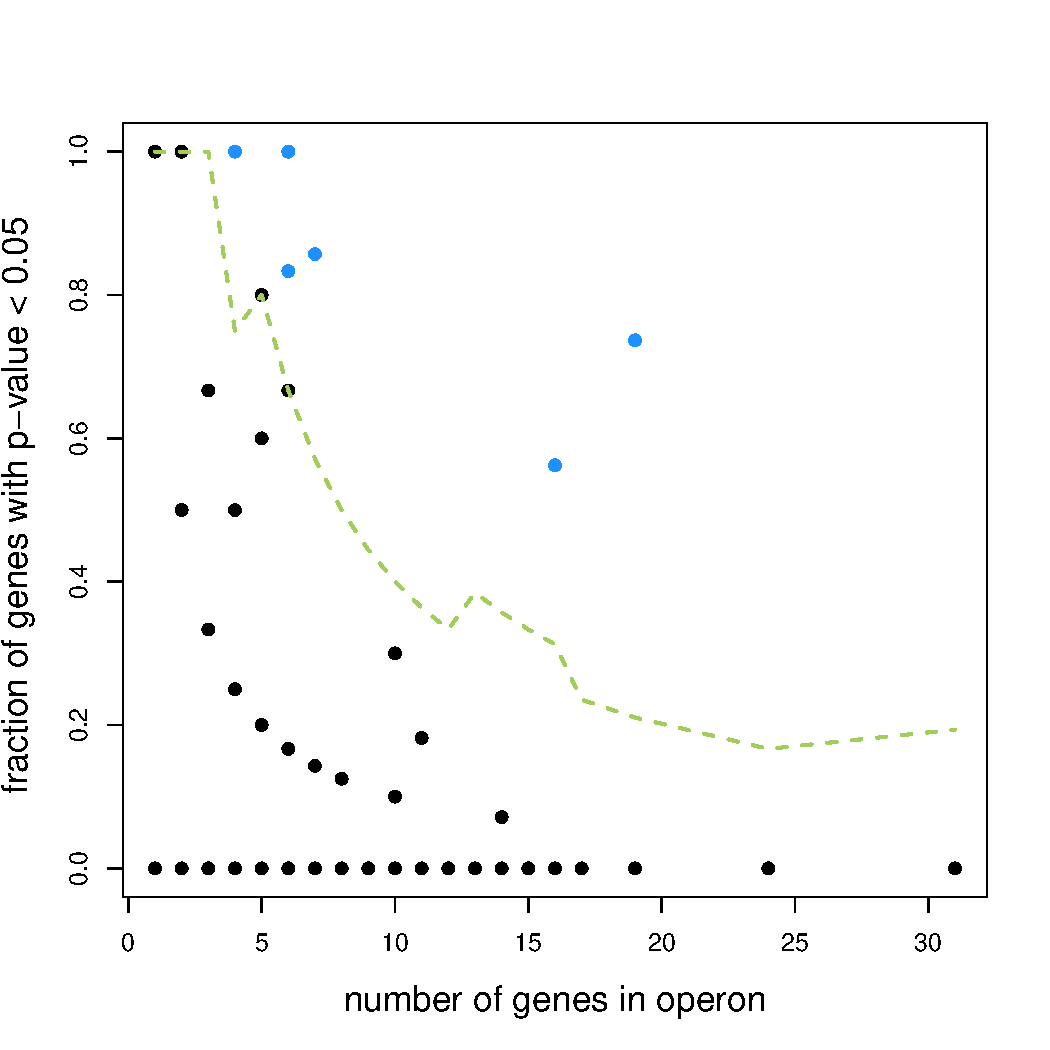
\includegraphics [width=0.75\textwidth] {Dissertation/images/operons/statsignificant_operons.pdf}
    \caption{Зависимость доли генов в оперонах, с уровнем значимости p-value < 0.05, от количества генов входящих в оперон. Пунктирная линия показывает максимальные значения, полученные при проведении 10000 случайных соотнесений генов и оперонов.}
    \label{img:operons_shuffle}
\end{figure}

Так, например, оперон утилизации пропандиола состоит из 19 генов, из которых 14 генов (74\%) имеют p-value < 0.05 в точном тесте Фишера. При проведении 10000 случайных пермутаций уровней значимости по генам, в данном опероне в среднем наблюдалось 3\% генов, а максимальная доля составила 21\%. Таким образом, можно сделать вывод, что повышенная представленность данного оперона в изолятах из пациентов, но не здоровых людей, не является случайным наблюдением. Полный список оперонов, определенных как значимо чаще встречающихся у изолятов из пациентов с болезнью Крона приведен в таблице~\ref{tbl:ops1}. 

\begin{table}[htbp]
\centering
\caption{Список оперонов статистически значимо пере-представленных в группе штаммов \textit{E. coli} изолированных из пациентов с болезнью Крона. N - количество генов, Pobs - наблюдаемое количество пере-представленных генов в опероне, Pmean - среднее количество перепредставленных генов при случайных пермутациях, Pmax - максимальное количество перепредставленных генов при случайных пермутациях.}
\label{tbl:ops1}
\begin{tabular}{|l|l|l|l|l|}
\hline
\textbf{N} & \textbf{Pobs} & \textbf{Pmean} & \textbf{Pmax} & \textbf{функция}                                  \\ \hline
4          & 1             & 0.03          & 0.75         & glyoxilate metabolism operon \\ \hline
6          & 0.83          & 0.02          & 0.67         & capsular assembly PAI IV LF82                              \\ \hline
6          & 1             & 0.02          & 0.67         & hemin uptake operon                                       \\ \hline
7          & 0.86          & 0.03          & 0.57         & sorbose uptake and utilization                             \\ \hline
16         & 0.56          & 0.02          & 0.31         & prophage I LF82                                            \\ \hline
19         & 0.74          & 0.03          & 0.21         & propanediol utilization operon                         \\ \hline
\end{tabular}
\end{table}

Исходный код программ, определяющих опероны, статистически значимо чаще встречающихся у изолятов, полученных от пациентов с болезнью Крона, доступен в репозитории \url{https://github.com/paraslonic/Rakitina_etal_Crohn_paper/blob/master/operonPval/}.


\newpage

\section{Участие в работе}

Результаты, описанные в разделах 4.1, 4.5, 4.7 данной главы были получены при участии Д. Н. Конанова.

Результаты, описанные в разделе 4.7 данной главы были получены также при участии Д. Е. Федорова и Р.И. Верещагина.

Результаты, описанные в разделе 4.3 данной главы были получены при участии И. С. Осмоловского.

Результаты, описанные в разделе 4.8 данной главы были получены при участии Д. В. Ракитиной и С. К. Гарушянц. 
